% Author         : Manuel Lippert
% Version        : 1.1
% Created on     : 11.06.2023
% Last Edited on : 11.06.2023

%%%%%%%%%%%%%%%%%%%%%%%%%%%%%%%%%%%%%%%%%%%%%%%%%%%%%%%%%%%%%%%%%%%%%%%%%%%
%                    !!! Compile with LuaLaTex !!!
%%%%%%%%%%%%%%%%%%%%%%%%%%%%%%%%%%%%%%%%%%%%%%%%%%%%%%%%%%%%%%%%%%%%%%%%%%%

\documentclass[compress,aspectratio=1610,noflama]{beamer}

%--------------------------------------------------------------------------
% Theme
%--------------------------------------------------------------------------

\usepackage{theme/beamerthemefancy}
\usetheme{fancy}

\usepackage{theme/dtklogos} % must be loaded after theme

%--------------------------------------------------------------------------
% Common packages
%--------------------------------------------------------------------------

\usepackage[english]{babel}
\usepackage{graphicx}
\usepackage{multicol}
\usepackage{multimedia}
\usepackage{media9}
\usepackage{hyperref}
\usepackage{tabularx}
\usepackage{tikz}
\usepackage{booktabs}
\usepackage{soul}
\usepackage{multirow}
\usepackage{xcolor}

%--------------------------------------------------------------------------
% Inputs
%--------------------------------------------------------------------------

\definecolor{Notablue}{HTML}{3498DB}		%Theoretische Physik
\definecolor{Notared}{HTML}{CF366C}			%Mathematik
\definecolor{Notagreen}{HTML}{19B092}		%Experimentalphysik
\definecolor{Notaorange}{HTML}{FA9D00}		%Chemie/Wahlfach nicht physikalisch
\definecolor{Notagrey}{HTML}{979690}		%Praktikum
\definecolor{Notalavendel}{HTML}{9DBBD8}	%Wahlfächer physikalisch
\definecolor{SPKred}{HTML}{E60005}

\definecolor{codegreen}{rgb}{0,0.6,0}
\definecolor{codegrey}{HTML}{979690}
\definecolor{codepurple}{rgb}{0.58,0,0.82}
\definecolor{codebackground}{gray}{0.92}

\definecolor{Ubtgreen}{RGB}{69, 155, 113}
\usepackage{tikz}
\usetikzlibrary{shapes.geometric, arrows}

\tikzstyle{startstop} = [
    rectangle, rounded corners, 
    minimum width=3cm, 
    minimum height=1cm,
    text centered,  
    align=center,
    fill=Notagreen!30
]

\tikzstyle{error} = [
    rectangle, rounded corners, 
    minimum width=3cm, 
    minimum height=1cm,
    text centered,  
    fill=Notagrey!30
]

\tikzstyle{init} = [
    rectangle, rounded corners, 
    minimum width=3cm, 
    minimum height=1cm, 
    text centered, 
    %draw=black, 
    fill=Notablue!30
]

\tikzstyle{process} = [
    rectangle, rounded corners, 
    minimum width=3cm, 
    minimum height=1cm, 
    text centered, 
    %draw=black, 
    fill=Notaorange!30
]

\tikzstyle{decision} = [
    diamond,
    aspect=3,
    minimum width=2.5cm, 
    minimum height=1.5cm, 
    text centered, 
    %draw=black, 
    fill=Notared!30
]

\tikzstyle{arrow} = [
    thick,
    ->,
    >=stealth
]
% Variables for quicker writing

% ExB Shortcuts
\newcommand{\wexb}{\omega_{\mathrm{\:E \times B}}}
\newcommand{\hatwexb}{\widehat{\omega}_{\mathrm{\:E \times B}}}
\newcommand{\exb}{\mathrm{\:E}\times\mathrm{B}}
%\newcommand{\hatwexbampvec}{|\hatwexb|_\mathbf{n}}
\newcommand{\hatwexbamp}{|\hatwexb|_{\nzf}}

\newcommand{\rlt}{R/L_T}

% Larmor Radius
%\newcommand{\rhoth}{\rho_\mathrm{th}}
\newcommand{\rhoth}{\rho_{\mathrm{th}}}
\newcommand{\rhost}{\rho_\star}

% Fields
\newcommand{\Epar}{E_{1\parallel}}
\newcommand{\gaEpar}{\ga{E}_{1\parallel}}

\newcommand{\gaE}{\ga{\vect{E}}}

\newcommand{\Bpar}{B_{1\parallel}}
\newcommand{\gaBpar}{\ga{B}_{1\parallel}}
\newcommand{\Bperp}{B_{1\perp}}
\newcommand{\gaBperp}{\ga{B}_{1\perp}}

\newcommand{\gaPhi}{\ga{\Phi}_1}

% Positions
\newcommand{\x}{\vect{x}}
\newcommand{\X}{\vect{X}}
\newcommand{\Xgy}{\vect{X}}

\newcommand{\rrho}{\vect{r}}

% Density
\newcommand{\nReq}{n_{R_0}}

% Vector Potentials
\newcommand{\A}{\vect{A}}
\newcommand{\gaA}{\ga{\A}_1}
\newcommand{\Apar}{A_{1\parallel}}
\newcommand{\gaApar}{\ga{A}_{1\parallel}}
\newcommand{\gaAperp}{\ga{A}_{1\perp}}

% Current
\newcommand{\vecj}{\vect{j}}

% Velocities
\newcommand{\velo}{\vect{v}}
\newcommand{\vecb}{\vect{b}}
\newcommand{\vpar}{v_\parallel}
\newcommand{\vperp}{\vect{v}_\perp}
\newcommand{\vchi}{\vect{v}_\chi}
\newcommand{\vD}{\vect{v}_\mathrm{D}}
\newcommand{\vth}{v_\mathrm{th}}

\newcommand{\ueq}{\vect{u}_0}
\newcommand{\upar}{u_\parallel}

% Distribution Functions
\newcommand{\fm}{F_\mathrm{M}}
% \newcommand{\df}{\delta \! f^{\mathrm{gy}}}
% \newcommand{\fgy}{f^{\mathrm{gy}}}
% \newcommand{\fgc}{f^{\mathrm{gc}}}
\newcommand{\fgy}{F}
\newcommand{\fgc}{F^\mathrm{gc}}
\newcommand{\df}{\fgy_1}

% Wavenumbers
\newcommand{\kperp}{k_\perp}
\newcommand{\kpar}{k_\parallel}

% Centrifugal energy
\newcommand{\cfen}{\mathcal{E}}

% Right hand side Vlasov
\newcommand{\vlaright}{\mathcal{V}}

% Reference values
\newcommand{\rhoref}{\rho_\mathrm{ref}}
\newcommand{\rhothref}{\rho_{\mathrm{th},\mathrm{ref}}}
\newcommand{\mref}{m_\mathrm{ref}}
\newcommand{\nref}{n_\mathrm{ref}}
\newcommand{\Tref}{T_\mathrm{ref}}
\newcommand{\Rref}{R_\mathrm{ref}}
\newcommand{\vthref}{v_{\mathrm{th},\mathrm{ref}}}
\newcommand{\Bref}{B_\mathrm{ref}}
\newcommand{\betaref}{\beta_\mathrm{ref}}

% Normalize values
\newcommand{\RN}{R_\mathrm{N}}
\newcommand{\BN}{B_\mathrm{N}}
\newcommand{\tN}{t_\mathrm{N}}
\newcommand{\kN}{k_\mathrm{N}}
\newcommand{\kperpN}{k_{\perp \mathrm{N}}}
\newcommand{\kparN}{k_{\parallel \mathrm{N}}}
\newcommand{\muN}{\mu_\mathrm{N}}
\newcommand{\vparN}{v_{\parallel \mathrm{N}}}
\newcommand{\OmegaN}{\Omega_\mathrm{N}}
\newcommand{\PhiN}{\Phi_{1 \mathrm{N}}}
\newcommand{\AparN}{A_{1\parallel \mathrm{N}}}
\newcommand{\BparN}{B_{1\parallel \mathrm{N}}}
\newcommand{\EparN}{E_{1\parallel \mathrm{N}}}
\newcommand{\fgyN}{\fgy_\mathrm{N}}
\newcommand{\fmN}{F_{\mathrm{M} \mathrm{N}}}
\newcommand{\betaN}{\beta_\mathrm{N}}
\newcommand{\cfenN}{\mathcal{E}_\mathrm{N}}
\newcommand{\vlarightN}{\vlaright_\mathrm{N}}

\newcommand{\nabperpN}{\nabla_{\!\perp \mathrm{N}}}
\newcommand{\nabparN}{\nabla_{\!\parallel \mathrm{N}}}

% Relative values
\newcommand{\mR}{m_\mathrm{R}}
\newcommand{\nR}{n_\mathrm{R}}
\newcommand{\TR}{T_\mathrm{R}}
\newcommand{\vthR}{v_{\mathrm{th} \mathrm{R}}}

% Fourier Trafo values (normalize, relative)
\newcommand{\FPhi}{\widehat{\Phi}_{1}}
\newcommand{\FBpar}{\widehat{B}_{1\parallel}}
\newcommand{\FApar}{\widehat{A}_{1\parallel}}
\newcommand{\FEpar}{\widehat{E}_{1\parallel}}

\newcommand{\FPhiN}{\widehat{\Phi}_{1 \mathrm{N}}}
\newcommand{\FBparN}{\widehat{B}_{1\parallel \mathrm{N}}}
\newcommand{\FAparN}{\widehat{A}_{1\parallel \mathrm{N}}}
\newcommand{\FEparN}{\widehat{E}_{1\parallel \mathrm{N}}}

\newcommand{\Ffgy}{\widehat{\fgy}}
\newcommand{\FfgyN}{\widehat{\fgy}_\mathrm{N}}
\newcommand{\Fvlaright}{\widehat{\vlaright}}
\newcommand{\FvlarightN}{\widehat{\vlaright}_\mathrm{N}}

% Differentials
\newcommand{\dx}{\mathrm{d}\vect{x}}
\newcommand{\dX}{\mathrm{d}\vect{X}}

\newcommand{\dvelo}{\mathrm{d}\vect{v}}
\newcommand{\dvpar}{\mathrm{d}\vpar}
\newcommand{\dvparN}{\mathrm{d}\vparN}

\newcommand{\Dx}{\partial\vect{x}}
\newcommand{\Dv}{\partial\vect{v}}
\newcommand{\Dt}{\partial t}

\newcommand{\dz}{\mathrm{d}z}
\newcommand{\dZ}{\mathrm{d}Z}
\newcommand{\dt}{\mathrm{d}t}

\newcommand{\dtheta}{\mathrm{d}\theta}
\newcommand{\dmu}{\mathrm{d}\mu}
\newcommand{\dmuN}{\mathrm{d}\muN}

\newcommand{\nabperp}{\nabla_{\!\perp}}
\newcommand{\nabpar}{\nabla_{\!\parallel}}

% Literature
\newcommand{\source}{\textcolor{red}{(Source)}}

% Grid points
\newcommand{\Nsp}{N_\mathrm{sp}}
\newcommand{\Nmod}{N_\mathrm{mod}}
\newcommand{\Nx}{N_x}
\newcommand{\Ns}{N_s}
\newcommand{\Nmu}{N_\mu}
\newcommand{\Nvpar}{N_{v_\parallel}}
\usepackage{tikz}

\usetikzlibrary{mindmap,backgrounds}
\usetikzlibrary{decorations.pathmorphing}
\usetikzlibrary{decorations.markings}
\usetikzlibrary{arrows.meta,bending}
\usetikzlibrary{decorations.pathreplacing}

%--------------------------------------------------------------------------
% Functions
%--------------------------------------------------------------------------

% Vector Quantities bold
\newcommand{\vect}[1]{\boldsymbol{\mathbf{#1}}}

% Common Indexes in Gyrokinetics
\newcommand{\iref}[1]{#1_\mathrm{ref}}
\newcommand{\ith}[1]{#1_\mathrm{th}}

% Add _s to any Quantity with seperation into Species
\newcommand{\spec}[1]{#1_s}
\newcommand{\specN}[1]{#1_{\mathrm{N},s}}
\newcommand{\speccN}[2]{#1_{#2\mathrm{N},s}}
\newcommand{\specthN}[1]{#1_{\mathrm{th}\mathrm{N},s}}
\newcommand{\specR}[1]{#1_{\mathrm{R},s}}
\newcommand{\specthR}[1]{#1_{\mathrm{th}\mathrm{R},s}}
\newcommand{\specref}[1]{#1_{\mathrm{ref},s}}

\newcommand{\specc}[2]{#1_{#2,s}}
\newcommand{\speccrm}[2]{#1_{\mathrm{#2},s}}

% Gyroaverage Operator
\newcommand{\ga}[1]{\bar{#1}}
\newcommand{\gad}[1]{\langle#1\rangle}
% \newcommand{\tga}[1]{\mathcal{G}\!\left\{ #1 \right\}}
% \newcommand{\tgad}[1]{\mathcal{G}^\dagger\!\left\{ #1 \right\}}
\newcommand{\tga}[1]{\mathcal{G} #1}
\newcommand{\tgad}[1]{\mathcal{G}^\dagger #1}

% Optimize Spacing of integrals
\newcommand{\ints}{\int \!}
\newcommand{\intss}[2]{\int_{#1}^{#2} \!\!\!\!\!}

\newcommand{\highlight}[1]{
  \colorbox{Notared!50}{$\displaystyle#1$}}

\newcommand{\highlightt}[1]{
	\colorbox{Notared!0}{$\displaystyle#1$}}

\newcommand{\code}[1]{{\ttfamily\small{#1}}}

%--------------------------------------------------------------------------
% Variables
%--------------------------------------------------------------------------

\graphicspath{{../pictures/}}

\newcommand{\backgroundpicture}{evaluation/benchmark/f-version/fields/kthrho0.300_beta0.008_fields_f-version.pdf}
\newcommand{\backgroundxshift}{0.27\paperwidth}
\newcommand{\backgroundwidth}{0.7\paperwidth} 

\newcommand{\logopicture}{Uni_Logo_white_black}

%--------------------------------------------------------------------------
% Document
%--------------------------------------------------------------------------

\title{Mitigation of \\ the Cancellation Problem \\ in local gyrokinetic Simulations}
\subtitle{~}
\author{Manuel Lippert}
\institute{Theoretical Physics V}

\begin{document}

	\maketitle

	\section*{Motivation}
	\begin{frame}
		\frametitle{Motivation}

		\begin{center}
			\begin{itemize}
				\item <2-> In plasma physics the plasma beta $\beta$ is one of the fundamental dimensionless parameters
				% \item <3-> Electromagentic fields vanish in the limit $\beta \rightarrow 0$ \\ $\rightarrow$ Indicator for the relevance of electromagnetic effects
				\item <3-> Kinetic Models describes plasma in the 6D phase space through the Vlasov equation and Maxwell equations.
				\item <4-> \textbf{Cancellation Problem:} Limits gyrokinetic investigations to low plasma beta high perpendicular wave vectors $\kperp$
				\item <5-> New technique for global nonlinear simulations found to mitigate the cancellation problem by using an additional field equation
			\end{itemize}
			\bigskip
			\onslide<6-> \textbf{Is it possible to mitigate the cancellation problem in local gyrokinetic simulations with the introduction of a new field equation?}
		\end{center}
	\end{frame}

	\section*{Plasma Physics Basics}

	\begin{frame}
		\frametitle{Charged Particle Motion}

		\begin{center}
			\begin{tabular}{>{\onslide<2->}c<{\onslide}@{\hspace{0.5cm}} >{\onslide<2->}c<{\onslide}@{\hspace{0.5cm}} >{\onslide<2->}c<{\onslide}}
				\textbf{Lorentz force} & 
				\textbf{Electric force} & 
				\textbf{Inhomogeneous magnetic field} \\
				$F_{\perp, B} = |q| v_\perp B$ & 
				$F_{\parallel,E} = qE_\parallel$ & 
				$F_{\parallel,\nabla_{\!\parallel} B} = - \underbrace{\frac{mv^2_{\perp}}{2B}}_{\mu} \nabla_{\!\parallel} B$ \\
				% \usetikzlibrary{mindmap,backgrounds}
% \usetikzlibrary{decorations.pathmorphing}
% \usetikzlibrary{decorations.markings}
% \usetikzlibrary{arrows.meta,bending}

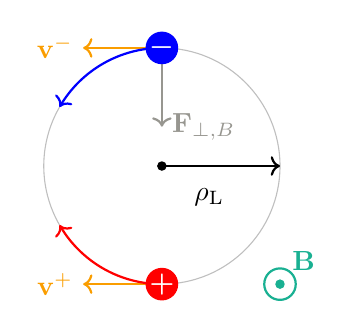
\begin{tikzpicture}
    % Circle
    \draw[lightgray] (0,0) circle (1.5);
    \filldraw (0,0) circle (1.5pt);
    % Force
    \draw[thick, Notagrey, <-] (90:0.5) node[right, Notagrey]{$\vect{F}_{\perp, B}$} -- ++ (90:1.0) node[coordinate] (x) {};
    % Larmor radius
    \draw[thick, black, ->] (0,0) -- ++(0:1.5);
    \draw (0.6,-0.4) node {$\rho_\mathrm{L}$};
    % Velocity
    \draw[thick,Notaorange, ->] (x) -- ++(180:1cm) node[left, Notaorange]{$\vect{v}^-$};
    \draw[thick,Notaorange, ->] (0,-1.5) -- ++(180:1cm) node[left, Notaorange]{$\vect{v}^+$};
    % Cyclontron freqency
    \draw[thick, ->, blue] (90:1.0*1.5) arc(90:150:1.0*1.5);
    \draw[thick, <-, red] (210:1.0*1.5) arc(210:270:1.0*1.5);
    % Charges
    \draw [fill=blue, blue] (x) circle (0.2) node[white, font=\boldmath]{$-$};
    \draw [fill=red, red] (0,-1.5) circle (0.2) node[white, font=\boldmath]{$+$};
    % Magnetic field
    \draw [thick, Notagreen] (1.5,-1.5) circle (0.2);
    \filldraw [Notagreen] (1.5,-1.5) circle (1.5pt);
    \draw (1.8,-1.2) node[Notagreen]{$\vect{B}$};
\end{tikzpicture} & 
				% \usetikzlibrary{mindmap,backgrounds}
% \usetikzlibrary{decorations.pathmorphing}
% \usetikzlibrary{decorations.markings}
% \usetikzlibrary{arrows.meta,bending}

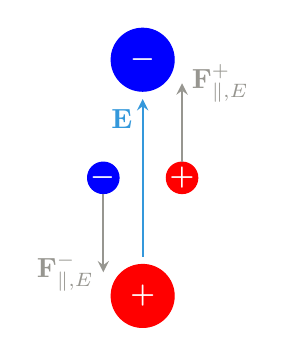
\begin{tikzpicture}
    % Charge
    \draw [fill=blue, blue] (0,1.5) circle (0.4) node[white, font=\boldmath]{$-$};
    \draw [fill=red, red] (0,-1.5) circle (0.4) node[white, font=\boldmath]{$+$};
    \draw [fill=blue, blue] (-0.5,0) circle (0.2) node[white, font=\boldmath]{$-$};
    \draw [fill=red, red] (0.5,0) circle (0.2) node[white, font=\boldmath]{$+$};
    % Electric field
    \draw[thick,Notablue, ->, >=stealth] (0,-1) -- (0,1) node[below left, Notablue] {$\vect{E}$};
    % Force
    \draw[thick, Notagrey, ->, >=stealth] (-0.5, -0.2) -- (-0.5, -1.2);
    \draw (-0.5, -1.2) node[left, Notagrey]{$\vect{F}^{-}_{\parallel,E}$};
    \draw[thick, Notagrey, ->, >=stealth] (0.5, 0.2) -- (0.5, 1.2);
    \draw (0.5, 1.2) node[right, Notagrey]{$\vect{F}^{+}_{\parallel,E}$};
\end{tikzpicture} & 
				% \usetikzlibrary{mindmap,backgrounds}
% \usetikzlibrary{decorations.pathmorphing}
% \usetikzlibrary{decorations.markings}
% \usetikzlibrary{arrows.meta,bending}

{
\def\ang{36}
\def\Rx{0.7}
\def\Ry{1.14}
\def\h{0.5}
\def\H{3}
\def\W{4}
\def\NB{2}

\begin{tikzpicture}

	\coordinate (O) at (0,0);
	\coordinate (N) at (0,0.24*\H);
	\coordinate (M) at (0,0.45*\H);
	\coordinate (B) at (\ang:\H);

	% Magnetic momentum (1/2)
	\draw [thick, Notared] (0,\Ry) arc (90:270:{\Rx} and {\Ry});
	% Magnetic field
	\foreach \i [evaluate={\y=(0.34*\H)*\i^2/\NB; \out=1*\i^2; \in=180+10*\i^2; \f=0.80-0.10*\i;}] in {1,...,\NB}{
	  \draw [thick, Notagreen, <-, >=stealth] (-0.95*\H, 0.7*\y/\H) to[out= \out,in= \in,looseness=0.8] (0.25*\W, \y);
	  \draw [thick, Notagreen, <-, >=stealth] (-0.95*\H,-0.7*\y/\H) to[out=-\out,in=-\in,looseness=0.8] (0.25*\W,-\y);
	}
	\node [Notagreen] at (0.26*\W,0.52*\H) {$\vect{B}$};
	% Force
	\draw [thick, Notagrey, ->, >=stealth] ( 95:{\Rx} and {\Ry}) --++ (-25:0.8*\Ry) node[right=0, Notagrey] {$\vect{F}_{\parallel,\nabla_{\!\parallel} B}$};
	\draw [thick, Notagrey, ->, >=stealth] (-95:{\Rx} and {\Ry}) --++ ( 25:0.8*\Ry) node[right=1, Notagrey] {$\vect{F}_{\parallel,\nabla_{\!\parallel} B}$};
	% Magnetic momentum (2/2)
	\draw [thick, Notared] (0,\Ry) arc (90:-90:{\Rx} and {\Ry});
	\draw [thick, Notared, ->, >=stealth] (0,0) --++ (-0.3*\W,0) node[left, Notared] {$\vect{\mu}$};
	% Particle
	\filldraw [Notablue] (-95:{\Rx} and {\Ry}) circle (2pt);
	\filldraw [Notablue] ( 95:{\Rx} and {\Ry}) circle (2pt);
	\draw (-3,1) node[above right, Notablue]{Particle};

\end{tikzpicture}} \\
				$\rho = \frac{m\vperp}{|q|B}~~~\omega_\mathrm{c} = \frac{|q|B}{m}$ & $\rhoth = \frac{m\vth}{|q|B}$ & $\vth=\sqrt{\frac{2T}{m}}$ \\
			\end{tabular}
		\end{center}
	\end{frame}
	
	\begin{frame}
		\frametitle{Drifts in the Guiding Center}
		\begin{center}
			\begin{tabular}{>{\onslide<2->}c<{\onslide} >{\onslide<3->}c<{\onslide} >{\onslide<3->}c<{\onslide}}
				{\boldmath $\exb$} \textbf{Drift} & 
				{\boldmath $\nabla B$} \textbf{Drift} & 
				\textbf{Curvature Drift} \\
				$\vect{v}_{E} = \frac{\vect{E}\times\vect{B}}{B^2}$ & 
				$\vect{v}_{\nabla B} = \frac{m v^2_{\perp}}{2 q}\frac{\vect{B}\times \nabla B}{B^3}$ & 
				$\vect{v}_{C} = \frac{m v^2_{\parallel}}{qB^2}\vect{B}\times \underbrace{\vect{C}}_{\frac{\nabla B}{B}} = \frac{m v^2_{\parallel}}{q} \frac{\vect{B}\times \nabla B}{B^3}$\\[1cm]
				% \usetikzlibrary{mindmap,backgrounds}
% \usetikzlibrary{decorations.pathmorphing}
% \usetikzlibrary{decorations.markings}
% \usetikzlibrary{arrows.meta,bending}

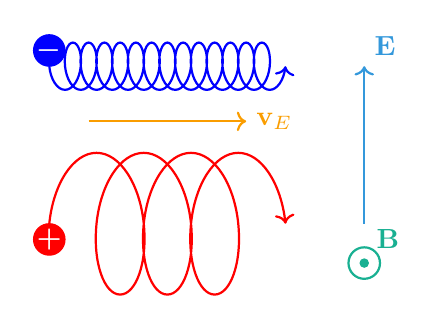
\begin{tikzpicture}
    % Electron
    \draw[thick,decoration={segment length=2mm, amplitude=0.3cm, coil},decorate,<-,blue] (3,0) -- (0,0);
    \draw [fill=blue, blue] (0,0.2) circle (0.2) node[white, font=\boldmath]{$-$};
    % Ion
    \draw[thick,decoration={coil, aspect = -0.5, amplitude = -0.9cm, segment length=6mm},decorate,<-,red] (3,-2) -- (0,-2);
    \draw [fill=red, red] (0,-2.2) circle (0.2) node[white, font=\boldmath]{$+$};
    % Electric field
    \draw[thick,Notablue, ->] (4,-2) -- (4,0) node[above right, Notablue]{$\vect{E}$};
    % Drift velocity
    \draw[thick,Notaorange, ->] (0.5,-0.7) -- (2.5,-0.7) node[right, Notaorange]{$\vect{v}_{E}$};
    % Magnetic field
    \draw [thick, Notagreen] (4,-2.5) circle (0.2);
    \filldraw [Notagreen] (4,-2.5) circle (1.5pt);
    \draw (4.3,-2.2) node[Notagreen]{$\vect{B}$};
\end{tikzpicture} & 
				\multicolumn{2}{>{\onslide<3->}c<{\onslide}}{% \usetikzlibrary{mindmap,backgrounds}
% \usetikzlibrary{decorations.pathmorphing}
% \usetikzlibrary{decorations.markings}
% \usetikzlibrary{arrows.meta,bending}

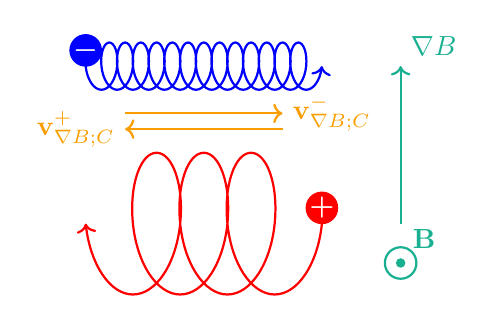
\begin{tikzpicture}
    % Electron
    \draw[thick,decoration={segment length=2mm, amplitude=0.3cm, coil},decorate,<-,blue] (3,0) -- (0,0);
    \draw [fill=blue, blue] (0,0.2) circle (0.2) node[white, font=\boldmath]{$-$};
    % Ion
    \draw[thick,decoration={coil, aspect = -0.5, amplitude = -0.9cm, segment length=6mm},decorate,<-,red] (0,-2) -- (3,-2);
    \draw [fill=red, red] (3,-1.8) circle (0.2) node[white, font=\boldmath]{$+$};
    % Grad B field
    \draw[thick,Notagreen, ->] (4,-2) -- (4,0) node[above right, Notagreen]{$\nabla B$};
    % Drift velocity
    \draw[thick,Notaorange, ->] (0.5,-0.6) -- (2.5,-0.6) node[right, Notaorange]{$\vect{v}^{-}_{\nabla B;C}$};
    \draw[thick,Notaorange, <-] (0.5,-0.8) node[left, Notaorange]{$\vect{v}^{+}_{\nabla B;C}$} -- (2.5,-0.8);
    % Magnetic field
    \draw [thick, Notagreen] (4,-2.5) circle (0.2);
    \filldraw [Notagreen] (4,-2.5) circle (1.5pt);
    \draw (4.3,-2.2) node[Notagreen]{$\vect{B}$};
\end{tikzpicture}} \\
			\end{tabular}
		\end{center}
	\end{frame}

	\begin{frame}
		\frametitle{Plasma Beta}

		\begin{center}
			% \only<2>{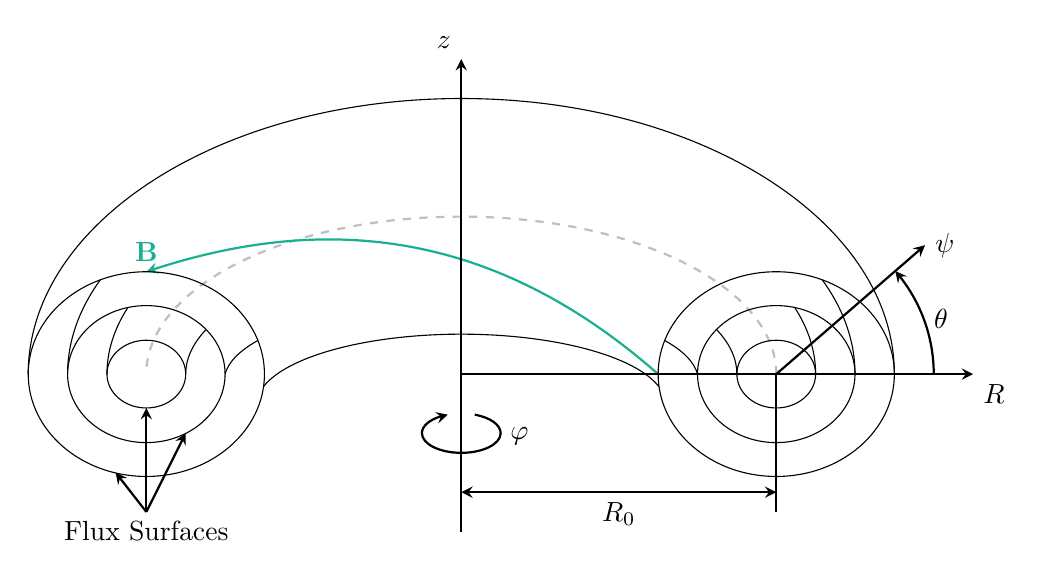
\begin{tikzpicture}
    
    % Torus tilted with 30 Degree -> Radius y = Radius x * 1/2
    % Torus Line Radius -> Radius x * 1/sqrt(2)

    % Elipse
    \draw[thick, lightgray, dashed] (4,0.0) arc (0:180:4 and 2);

    % Magnetic Field
    \draw[thick, ->, >=stealth, Notagreen] (2.5, 0) to[bend right] (-4,1.3) node [above, Notagreen] {$\vect{B}$};

    % Coordinate System
    \draw[thick, ->, >=stealth] (0,-2) -- (0,4) node[above left]{$z$}; 
    \draw[thick, ->, >=stealth] (0,0) -- (6.5,0) node[below right]{$R$};

    % Torus 1
    \draw (4,0) circle (0.5 and 0.43);
    \draw (-4,0) circle (0.5 and 0.43);
    
    \draw (4,0) + (0.5, 0)  arc (0:19.8:4.5 and 2.5);
    \draw (-4,0) + (-0.5, 0)  arc (180:160.2:4.5 and 2.5);
    \draw (-4,0) + (0.5, 0)  arc (180:158:3.5 and 1.5);
    \draw (4,0) + (-0.5, 0)  arc (0:22:3.5 and 1.5);

    % Torus 2
    \draw (4,0) circle (1.0 and 0.87);
    \draw (-4,0) circle (1.0 and 0.87);

    \draw (4,0) + (1.0, 0)  arc (0:23.5:5.0 and 3.0);
    \draw (-4,0) + (-1.0, 0)  arc (180:156.5:5.0 and 3.0);
    \draw (-4,0) + (1.0, 0)  arc (175:149:3.01 and 1.0);
    \draw (4,0) + (-1.0, 0)  arc (5:31:3.01 and 1.0);

    % Torus 3
    \draw (4,0) circle (1.5 and 1.3);
    \draw (-4,0) circle (1.5 and 1.3);

    \draw (4,0) + (1.5, 0)  arc (0:180:5.5 and 3.5);
    \draw (0,0) + (2.51,-0.16) arc (15:165:2.6 and 0.9);
    
    % Coordinates
    \draw[thick, ->, >=stealth] (4,0) ++ (0:2) arc (0:40.9:2) node[midway, right]{$\theta$};
    \draw[thick, ->, >=stealth] (4,0) -- ++ (40.9:2.5) node[right]{$\psi$};

    \draw[thick] (0,-1.0) arc (-90:70:0.5 and 0.25) node[midway, right]{$\varphi$};
    \draw[thick, ->, >=stealth] (0,-1.0) arc (-90:-250:0.5 and 0.25);

    \draw[thick] (4,0) -- (4,-1.75);
    \draw[thick, <->, >=stealth] (0,-1.5) -- node[midway, below] {$R_0$} (4,-1.5); 

    \draw[thick, ->, >=stealth] (-4,-1.75) -- (-4.00, -0.43);
    \draw[thick, ->, >=stealth] (-4,-1.75) -- (-3.50, -0.75);
    \draw[thick, ->, >=stealth] (-4,-1.75) -- (-4.39, -1.25);
    \draw (-4,-1.75) node[below]{Flux Surfaces};


\end{tikzpicture}}
			\onslide<2-> $\beta = \frac{\overbrace{nT}^\mathrm{plasma~pressure}}{\underbrace{B^2/2\mu_0}_\mathrm{magnetic~field~pressure}}$
			\bigskip
			\begin{itemize}
				\item <3-> Characterizes quality of confinement (Best confinement for $\beta < 1$)
				\item <3-> Relevant for fusion rate ($\sim \beta^2$), MHD stability of a fusion device
				\item <3-> Indicator for the relevance of electromagnetic effects 
				\item <3-> Electromagentic fields vanish in the limit $\beta \rightarrow 0$
			\end{itemize}
		\end{center}
	\end{frame}

	\section*{Gyrokinetic Theory}

	\begin{frame}
		\frametitle{Gyrokinetic Ordering}

		\begin{center}
			\begin{itemize}
				\item <2-> Low frequency: $\omega/\omega_\mathrm{c} \ll 1$
				\item <2-> Anisotropy: $k_\parallel/k_\perp \ll 1$
				\item <2-> Strong Magnetization: $\rho/L_n \sim \rho/L_T \sim \rho/L_B \ll 1 \qquad L_G = G_0 \left(\frac{\mathrm{d}G_0}{\mathrm{dx}}\right)^{-1}$
				\item <2-> Small fluctuations: $\fgy_1 / \fgy_0 \ll 1$
			\end{itemize}

			\bigskip
			
			\onslide<3-> {
				\begin{gather*}
					\omega /\omega_\mathrm{c} \sim k_\parallel/k_\perp \sim \rho/L_n \sim \rho/L_T \sim \rho/L_B \sim \fgy_1/\fgy_0 \sim \epsilon_\delta \\
					\rhost = \frac{\rhothref}{L_B} = \frac{\mref \vthref}{e \Bref} \sim \epsilon_\delta
				\end{gather*}
			}
		\end{center}
	\end{frame}

	\begin{frame}
		\frametitle{Derivation of gyrokinetic equation}

		\begin{center}
			\only<4>{% \usetikzlibrary{mindmap,backgrounds}
% \usetikzlibrary{decorations.pathmorphing}
% \usetikzlibrary{decorations.markings}
% \usetikzlibrary{arrows.meta,bending}

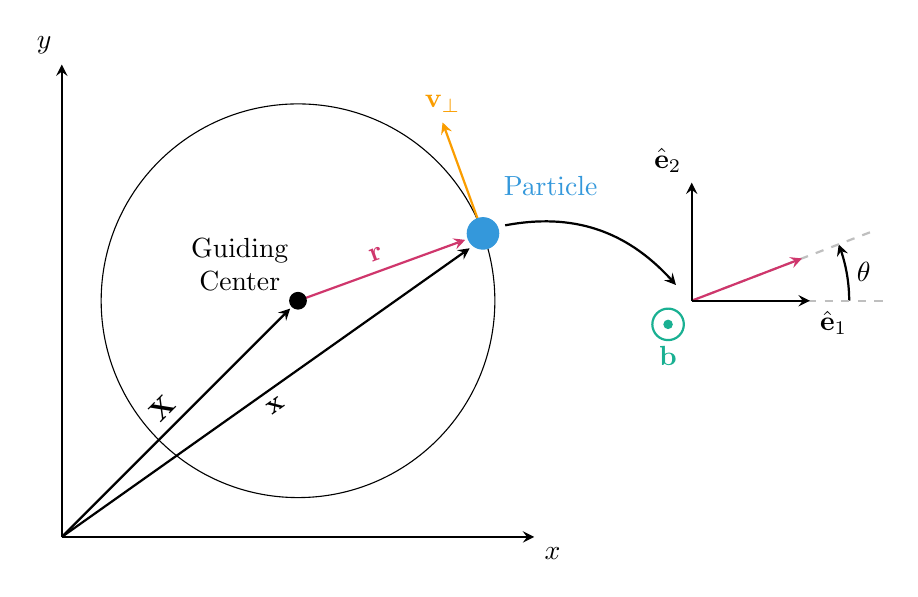
\begin{tikzpicture}

    % Coordinate System
    \draw[thick, ->, >=stealth] (-3,-3) -- (-3,3) node[above left]{$y$}; 
    \draw[thick, ->, >=stealth] (-3,-3) -- (3,-3) node[below right]{$x$};

    % Gyroangle
    \draw[thick, ->, >=stealth] (5,0) ++ (0:2) arc (0:21:2) node[midway, right]{$\theta$};
    \draw[thick, dashed, lightgray] (5,0) -- (7.5,0);
    \draw[thick, dashed, lightgray] (5,0) -- ++ (21:2.5);
    \draw[thick, black, ->, Notared, >=stealth] (5,0) -- ++ (21:1.5);

    % Unit Vecctor System
    \draw[thick, ->, >=stealth] (5,0) -- (5,1.5) node[above left]{$\hat{\vect{e}}_2$}; 
    \draw[thick, ->, >=stealth] (5,0) -- (6.5,0) node[below  right]{$\hat{\vect{e}}_1$}; 

    % Circle
    \draw (0,0) circle (2.5) node[above left, align=center]{Guiding \\ Center};
    
    % Velocity
    \draw[thick,Notaorange, ->, >=stealth] (20:2.5) -- ++(110:1.5cm) node[above, Notaorange]{$\vect{v}_\perp$};

    % Charges
    \draw [fill=Notablue,Notablue] (20:2.5) circle (0.2) node[right, above right, xshift = 4, yshift = 10, Notablue]{Particle};

    % Larmor radius
    \draw[thick, ->, >=stealth, Notared] (0,0) -- ++ (20:2.26) node[midway, above, Notared, sloped]{$\rrho$};

    % Position Vectors
    \draw[thick, black, ->, >=stealth] (-3,-3) -- (17:2.28) node[midway, below, sloped]{$\x$};
    \draw[thick, black, ->, >=stealth] (-3,-3) -- (-0.1,-0.1) node[midway, above, sloped]{$\X$};

    % Guiding Center
    \filldraw (0,0) circle (3pt);
    
    % Magnetic field
    \draw [thick, Notagreen] (4.7,-0.3) circle (0.2);
    \filldraw [Notagreen] (4.7,-0.3) circle (1.5pt);
    \draw (4.7,-0.7) node[Notagreen]{$\vect{b}$};

    % Coordinate System Vector
    \draw[thick, black, ->, >=stealth] (20:2.8) to[bend left] (4.8,0.2);

\end{tikzpicture}}
			\begin{itemize}
				\only<2-3,5-6>{
					\item Find fundamental one-form of the gyrocenter phase space \\
					\begin{gather*}
						\int \dt ~ L = \int \gamma
					\end{gather*}
				}
				\only<3,5-6>{
					\item Particle phase space $\{\x,\velo\}$ $\rightarrow$ guiding center $\{\X,\vpar, \mu, \theta\}$ $\rightarrow$ gyrocenter $\{\bar{\X},\bar{\vpar},\bar{\mu}\}$
					\begin{gather*}
						\Phi = \Phi_0 + \underbrace{\tilde{\Phi}_1 + \bar{\Phi}_1}_{\Phi_1} \qquad \A = \A_0 + \underbrace{\tilde{\A}_1 + \bar{\A}_1}_{\A_1}
					\end{gather*}
				}
				\only<6>{
					\item Vlasov Equation in gyrocenter phase space without collisions
					\begin{gather*}
						\frac{\partial \fgy}{\Dt} + \dot{\X} \cdot \frac{\partial \fgy}{\partial \vect{X}} + \dot{v}_\parallel \cdot \frac{\partial \fgy}{\partial v_\parallel} = 0
					\end{gather*}
				}
				\item <7-> Delta-$f$ approximation $F = F_0 + \df$
				\begin{gather*}
					\frac{\partial \df}{\Dt} + \dot{\X} \cdot \nabla \df + \dot{v}_\parallel \cdot \frac{\partial \df}{\partial v_\parallel} = \underbrace{- \dot{\X} \cdot \nabla \fgy_0 - \dot{v}_\parallel \frac{\partial \fgy_0}{\partial v_\parallel}}_S
				\end{gather*}
				\item <8> Maxwellian as equilibrium distribution $F_0 = \fm$ and $\dot{\X}$ and $\dot{\vpar}$ from Lagrangian
				\begin{gather*}
					\frac{\partial \df}{\Dt} + \dot{\X} \cdot \nabla \df - \frac{\vecb_0}{m} \cdot \left(Ze\nabla \Phi_0 + \mu \nabla B_0 - mR \Omega^2 \nabla R \right) \cdot \frac{\partial \df}{\partial v_\parallel} = S 
				\end{gather*}
				\begin{align*}
						S = -& (\vchi + \vD) \cdot \widetilde{\nabla} \fm - \frac{Z e \vpar}{T} \partial_t \gaApar \fm \\
						    -& \frac{\fm}{T} (\vpar \vecb_0 + \vD + \vBperp) \cdot (Z e \nabla \bar{\Phi} + \mu \nabla \gaBpar)
				\end{align*}
			\end{itemize}
		\end{center}
	\end{frame}

	\begin{frame}
		\frametitle{Derivation of Field Equations}
		
		\begin{center}
			\only<4-5>{\newcommand{\distance}{3cm}

\begin{tikzpicture}[node distance=2cm]

        \node (guidingcenter)  [startstop]                                         {Guiding Center Space};
        \node (vlasov)         [init, above of=guidingcenter, xshift= \distance]   {Vlasov Equation for $\fgy$};
        \node (moments)        [init, above of=guidingcenter, xshift=-\distance]   {Moments of $f$: $n(\x)$, $\vecj(\x)$};
        
        \draw [arrow] (vlasov)   -- (guidingcenter);
        \draw [arrow] (moments)  -- (guidingcenter);

\end{tikzpicture}
}
			\only<6>{% \usetikzlibrary{mindmap,backgrounds}
% \usetikzlibrary{decorations.pathmorphing}
% \usetikzlibrary{decorations.markings}
% \usetikzlibrary{arrows.meta,bending}

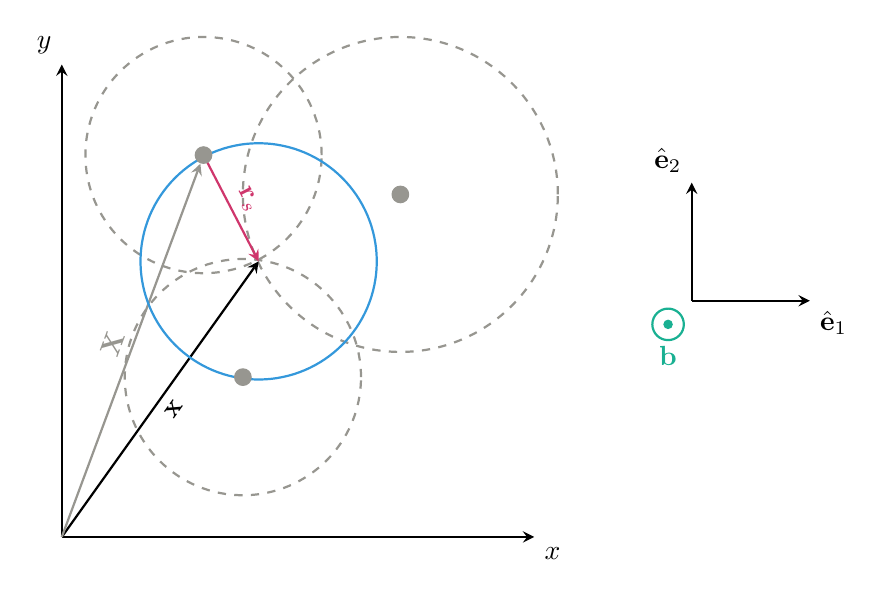
\begin{tikzpicture}

    % Coordinate System
    \draw[thick, ->, >=stealth] (-3,-3) -- (-3,3) node[above left]{$y$}; 
    \draw[thick, ->, >=stealth] (-3,-3) -- (3,-3) node[below right]{$x$};

    % Unit Vecctor System
    \draw[thick, ->, >=stealth] (5,0) -- (5,1.5) node[above left]{$\hat{\vect{e}}_2$}; 
    \draw[thick, ->, >=stealth] (5,0) -- (6.5,0) node[below  right]{$\hat{\vect{e}}_1$}; 

    % Circle
    \draw[thick, Notagrey, dashed] (-1.2,1.85)  circle (1.5);
    \draw[thick, Notagrey, dashed] (1.3,1.35)   circle (2);
    \draw[thick, Notagrey, dashed] (-0.7,-0.97) circle (1.5);

    % Larmor radius
    \draw[thick, ->, >=stealth, Notared] (-1.2,1.85) -- (-0.5,0.5) node[midway, above, Notared, sloped]{$\spec{\rrho}$};

    % Position Vectors
    \draw[thick, black, ->, >=stealth] (-3,-3) -- (-0.5,0.5) node[midway, below, sloped]{$\x$};
    \draw[thick, black, ->, >=stealth, Notagrey] (-3,-3) -- (-1.24,1.74) node[midway, above, sloped]{$\X$};
    
    % Magnetic field
    \draw [thick, Notagreen] (4.7,-0.3) circle (0.2);
    \filldraw [Notagreen] (4.7,-0.3) circle (1.5pt);
    \draw (4.7,-0.7) node[Notagreen]{$\vect{b}$};

    \draw[thick, Notablue] (-0.5,0.5) circle (1.5);

    % Guiding Center
    \filldraw[Notagrey] (-1.2,1.85)  circle (3pt);
    \filldraw[Notagrey] (1.3,1.35)   circle (3pt);
    \filldraw[Notagrey] (-0.7,-0.97) circle (3pt);

\end{tikzpicture}}

			\begin{itemize}
				\only<2-3>{
					\item Maxwell's equations
					\begin{align*}
						\spec{\sum} \spec{Z} e \, \spec{n} &= 0  &\qquad \nabla \times \vect{E}_1 &= - \frac{\partial \vect{B}_1}{\Dt}\\
						\nabla \cdot \vect{B}_1 &= 0 &\qquad \nabla \times \vect{B}_1 &= \mu_0 \spec{\sum} \spec{\vecj}
					\end{align*}
				}
				\only<3>{
					\item Moments of the distribution $f$
					\begin{gather*}
						n(\x) = \ints \dvelo ~ f(\x, \velo) \\
					j_\parallel = Ze \ints \dvelo ~ \vpar f(\x, \velo) \qquad \vecj_\perp = Ze \ints \dvelo ~ \vperp f(\x, \velo)
					\end{gather*}
				}
				\only<4-5>{\item Pullback transformation
				\begin{gather*}
					\fgc = \mathcal{P} \left\{ \fgy \right\} = \fgy \underbrace{- \frac{\fm}{T}\left(Ze \widetilde{\Phi}_1 - \mu \gaBpar\right)}_{\mathrm{Correction~Term}}
				\end{gather*}}
				\only<5>{
					\item Moments of the distribution $\fgc$
					\begin{align*}
						n &= \ints \dvelo ~ f(\x, \velo) = \frac{B_0}{m} \ints \dX\dvpar\dtheta\dmu ~ \delta(\X + \rrho - \x) \fgc \\
						j_\parallel &= Ze \ints \dvelo ~ \vpar f(\x, \velo)= \frac{Ze B_0}{m} \ints \dX\dvpar\dtheta\dmu ~ \delta(\X + \rrho - \x) \vpar \fgc \\
						\vecj_\perp &= Ze \ints \dvelo ~ \vperp f(\x, \velo) = \frac{Ze B_0}{m} \ints \dX\dvpar\dtheta\dmu ~ \delta(\X + \rrho - \x) \vperp \fgc
					\end{align*}
				}
				\item <7-> Coulomb's law \\ $\rightarrow \spec{\sum} \spec{Z} e \, \spec{n}  = 0 \rightarrow \Phi_1$
				\item <7-> Magnetic Compression \\ $\rightarrow \nabla^2 \Aperp = (\nabla \times \Bpar)_\perp = - \mu_0 \vecj_{1 \perp} \rightarrow \Bpar$
				\item <7-> Ampere's law \\ $\rightarrow \nabla^2 \Apar = - \mu_0 j_{1\parallel} \rightarrow \Apar$
				\onslide<8>{
					\begin{gather*}
						\kperpN^2 \FAparN = 2 \pi \BN \betaref\spec{\sum} \spec{Z} \specR{n} \specthR{v} \ints \dvparN\dmuN ~ \vparN J_0(\kperp \spec{\rho}) \speccN{\Ffgy}{1}
					\end{gather*}
				}
			\end{itemize}
		\end{center}
	\end{frame}

	\begin{frame}
		\frametitle{The Cancellation Problem}
		
		\begin{itemize}
			\only<2>{
				\item Gyrokinetic equation
				\begin{gather*}
					\highlightt{\frac{\partial \df}{\Dt}} + \dot{\X} \cdot \nabla \df - \frac{\vecb_0}{m} \cdot \left(Ze\nabla \Phi_0 + \mu \nabla B_0 - mR \Omega^2 \nabla R \right) \cdot \frac{\partial \df}{\partial v_\parallel} = S 
				\end{gather*}
				\begin{align*}
						S = -& (\vchi + \vD) \cdot \widetilde{\nabla} \fm -\highlightt{\frac{Z e \vpar}{T} \partial_t \gaApar \fm} \\
						    -& \frac{\fm}{T} (\vpar \vecb_0 + \vD + \vBperp) \cdot (Z e \nabla \bar{\Phi} + \mu \nabla \gaBpar)
				\end{align*}
			}
			\only<3>{
				\item Gyrokinetic equation
				\begin{gather*}
					\highlight{\frac{\partial \df}{\Dt}} + \dot{\X} \cdot \nabla \df - \frac{\vecb_0}{m} \cdot \left(Ze\nabla \Phi_0 + \mu \nabla B_0 - mR \Omega^2 \nabla R \right) \cdot \frac{\partial \df}{\partial v_\parallel} = S 
				\end{gather*}
				\begin{align*}
						S = -& (\vchi + \vD) \cdot \widetilde{\nabla} \fm -\highlight{\frac{Z e \vpar}{T} \partial_t \gaApar \fm} \\
						    -& \frac{\fm}{T} (\vpar \vecb_0 + \vD + \vBperp) \cdot (Z e \nabla \bar{\Phi} + \mu \nabla \gaBpar)
				\end{align*}
			}
			\only<4>{
				\item Modified distribution function
				\begin{gather*}
					g = \df + \frac{Ze \vpar}{T} \gaApar \fm
				\end{gather*}
				\item Modified gyrokinetic equation
				\begin{gather*}
					\highlightt{\frac{\partial g}{\Dt} + \vchi \cdot \nabla g} + (\vpar \vecb_0 + \vD) \cdot \nabla \df - \frac{\vecb_0}{m} \cdot (Z e \nabla \Phi_0 + \mu \nabla B_0 - m R \Omega^2 \nabla R) \frac{\partial \df}{\partial \vpar} = S \\
					S = - (\vchi + \vD) \cdot \tilde{\nabla} \fm - \highlightt{\frac{\fm}{T} (\vpar \vecb_0 + \vD) \cdot (Ze \nabla \bar{\Phi} + \mu \nabla \gaBpar)}
				\end{gather*}
			}
			\only<5>{
				\item Modified distribution function
				\begin{gather*}
					g = \df + \frac{Ze \vpar}{T} \gaApar \fm
				\end{gather*}
				\item Modified gyrokinetic equation
				\begin{gather*}
					\highlight{\frac{\partial g}{\Dt} + \vchi \cdot \nabla g} + (\vpar \vecb_0 + \vD) \cdot \nabla \df - \frac{\vecb_0}{m} \cdot (Z e \nabla \Phi_0 + \mu \nabla B_0 - m R \Omega^2 \nabla R) \frac{\partial \df}{\partial \vpar} = S \\
					S = - (\vchi + \vD) \cdot \tilde{\nabla} \fm - \highlight{\frac{\fm}{T} (\vpar \vecb_0 + \vD) \cdot (Ze \nabla \bar{\Phi} + \mu \nabla \gaBpar)}
				\end{gather*}
			}
			\only<6>{
				\item Adjusted Ampere's Law
				\begin{align*}
					&\left(\kperpN^2 + \betaref \spec{\sum} \frac{\spec{Z^2}\specR{n}}{\specR{m}} \Gamma_0(\spec{b}) e^{-\specN{\cfen}/\specR{T}} \right) \FAparN = \\
					& 2\pi\BN \betaref \spec{\sum} \spec{Z} \specR{n} \specthR{v} \ints \dvparN \dmuN ~ \vparN J_0(\kperp \spec{\rho}) \specN{\widehat{g}}
				\end{align*}
			}
			\only<7>{
				\item Adjusted Ampere's Law
				\begin{align*}
					&\left(\kperpN^2 + \highlight{\betaref \spec{\sum} \frac{\spec{Z^2}\specR{n}}{\specR{m}} \Gamma_0(\spec{b}) e^{-\specN{\cfen}/\specR{T}}} \right) \FAparN = \\
					& 2\pi\BN \betaref \spec{\sum} \spec{Z} \specR{n} \specthR{v} \ints \dvparN \dmuN ~ \vparN J_0(\kperp \spec{\rho}) \speccN{\Ffgy}{1} \\
					& + \highlight{2\pi\BN \betaref \spec{\sum} \spec{Z} \specR{n} \specthR{v} \ints \dvparN \dmuN ~ \vparN^2 J_0^2(\kperp \spec{\rho}) \frac{Ze \vth}{\Tref\TR} \fmN} \FAparN 
				\end{align*}
			}
			\item <7> Error scales with $\sim {\beta}/{\kperp^2}$
		\end{itemize}
	
	\end{frame}

	\begin{frame}
		\frametitle{Mitigation of the Cancellation Problem - Faraday's Law} 
		
		\begin{center}
			\begin{itemize}
				\only<2-3>{
					\item Faraday's law
					\begin{gather*}
						\rightarrow \Epar = - \frac{\partial \Apar}{\Dt} \rightarrow \nabla^2 \left( - \frac{\partial \Apar}{\Dt}\right) = \mu_0 \frac{\partial j_{1\parallel}}{\Dt} \rightarrow \Epar
					\end{gather*}
					\begin{gather*}
						\kperpN^2 \underbrace{\left(- \frac{\partial \FAparN}{\partial \tN}\right)}_{\FEparN} = - 2 \pi \BN \betaref\spec{\sum} \spec{Z} \specR{n} \specthR{v} \ints \dvparN\dmuN ~ \vparN J_0(\kperp \spec{\rho}) \frac{\partial \speccN{\Ffgy}{1}}{\partial \tN} 
					\end{gather*}
				}
				\only<3>{
					\item Replacing the time derivative of the gyrocenter distribution function
					\begin{gather*}
						\frac{\partial \df}{\Dt} = \rhs - \frac{Ze \vpar}{T} \frac{\partial \gaApar}{\Dt} \fm = \rhs + \frac{Ze \vpar}{T} \gaEpar \fm
					\end{gather*}
				}
				\only<4-5>{
					\item Field Equation for induced electric field $\Epar$
					\begin{align*}
						&\left(\kperpN^2 + \betaref \spec{\sum} \frac{\spec{Z^2}\specR{n}}{\specR{m}} \Gamma_0(\spec{b}) e^{-\specN{\cfen}/\specR{T}} \right) \FEparN = \\
						&- 2\pi\BN \betaref \spec{\sum} \spec{Z} \specR{n} \specthR{v} \ints \dvparN \dmuN ~ \vparN J_0(\kperp \spec{\rho}) \specN{\Frhs}
					\end{align*}
				}
				\only<5>{
					\item New source term in gyrokinetic equation
					\begin{gather*}
						\frac{\partial \df}{\Dt} + \dot{\X} \cdot \nabla \df - \frac{\vecb_0}{m} \cdot \left(Ze\nabla \Phi_0 + \mu \nabla B_0 - mR \Omega^2 \nabla R \right) \cdot \frac{\partial \df}{\partial v_\parallel} = S 
					\end{gather*}
					\begin{align*}
							S = -& (\vchi + \vD) \cdot \widetilde{\nabla} \fm - \highlight{\frac{Z e \vpar}{T} \gaEpar \fm} \\
							    -& \frac{\fm}{T} (\vpar \vecb_0 + \vD + \vBperp) \cdot (Z e \nabla \bar{\Phi} + \mu \nabla \gaBpar)
					\end{align*}
				}
			\end{itemize}
		\end{center}
	\end{frame}

	\section*{Mitigation in local Simulations}

	\begin{frame}
		\frametitle{Implementation of Faraday's Law}
		
		\onslide <2-> {\begin{tikzpicture}[node distance=2cm]

    \node (dist)        [dist, yshift=-0.75cm]                        {$\df^i$};
    \node (fields)      [terms, xshift= 3.5cm,  minimum width=4.5cm]  {Linear Terms};
    \node (nonfields)   [terms, xshift= 4.75cm, yshift = -1.5cm]      {Nonlinear \\ Terms};
    \node (rhs)         [dist,   xshift= 7cm, yshift=-0.75cm]         {$\rhs^{i+1}$};
    \node (distp)       [dist,   xshift= 11.5cm, yshift = -1.5cm]     {$\df^{i+1}$};
    \node (eparcorrect) [correct,xshift= 9.25cm, yshift = -1.5cm]     {$\Epar$ \\ Correct};
    \node (aparcorrect) [correct,xshift= 2.25cm, yshift = -1.5cm]     {$\Apar$ \\ Correct};
    \node (addfields)   [fields, xshift= 7cm, yshift = -2.25cm]       {$\Epar^{i+1}$};

        
    \draw [curly] (aparcorrect.south west) -- (fields.north west);
    \draw [curly] (fields.north east)      -- (nonfields.south east);
    \draw [arrow] (rhs)                    -- (addfields);
    \draw [curly] (rhs.north east)         -- (addfields.south east);
    \draw [arrow] (eparcorrect)            -- (distp);
    \draw [arrow] (aparcorrect)            -- (nonfields);


\end{tikzpicture}}

		\begin{itemize}
			\item <2-> {\gkw} calculates the modified distribution $g$ (g-version)\\
			$\rightarrow$ Switch to the calculation of the gyrocenter distribution $\df$ (f-version)
			\item <3-> Input switch \code{nlepar}
			\item <4-> Apply $\Apar$ correction on $\df$ for the calculation of the nonlinear terms
			\item <5-> Calculation of Faraday's law in an additional subroutine with $\rhs$ 
			\item <6-> Apply $\Epar$ correction on $\rhs$ for the calculation of $\df$
		\end{itemize}
	
	\end{frame}

	\begin{frame}
		\frametitle{Benchmark of the f-version}
		
		\only<2>{
			\begin{center}
				\begin{itemize}
					\item Flux-tube version of {\gkw} with field aligned Hamada coordinates $\{s,\psi, \zeta, \vpar, \mu \}$
					\item Cyclone base case (CBC) beta scan for 
					\begin{gather*}
						\beta \in [0.0,~0.2,~0.4,~0.6,~0.8,~1.0,~1.1,~1.2,~1.4,~1.6,~1.8,~2.0,~2.2]\,\%
					\end{gather*}
					\item Kinetic electrons (\code{adiabatic\_electrons} = \code{.false.})
					\item $k_\zeta \rho = 0.3$ (Maximum of the nonlinear transport spectrum)
				\end{itemize}
				\bigskip
				\begin{tabular}{c c c | c c c c c c c}
					\code{DTIM} & \code{NTIME} & \code{NAVERAGE} & $\Nmod$ & $\Nx$ & $\Ns$ & $\Nvpar$ & $\Nmu$ & $\Nsp$ & \code{nperiod} \\ \hline
					0.01 & 2000 & 100 & 1 & 1 & 288 & 64 & 16 & 2 & 5
				\end{tabular}
			\end{center}
		}

		\centering
		\only<3>{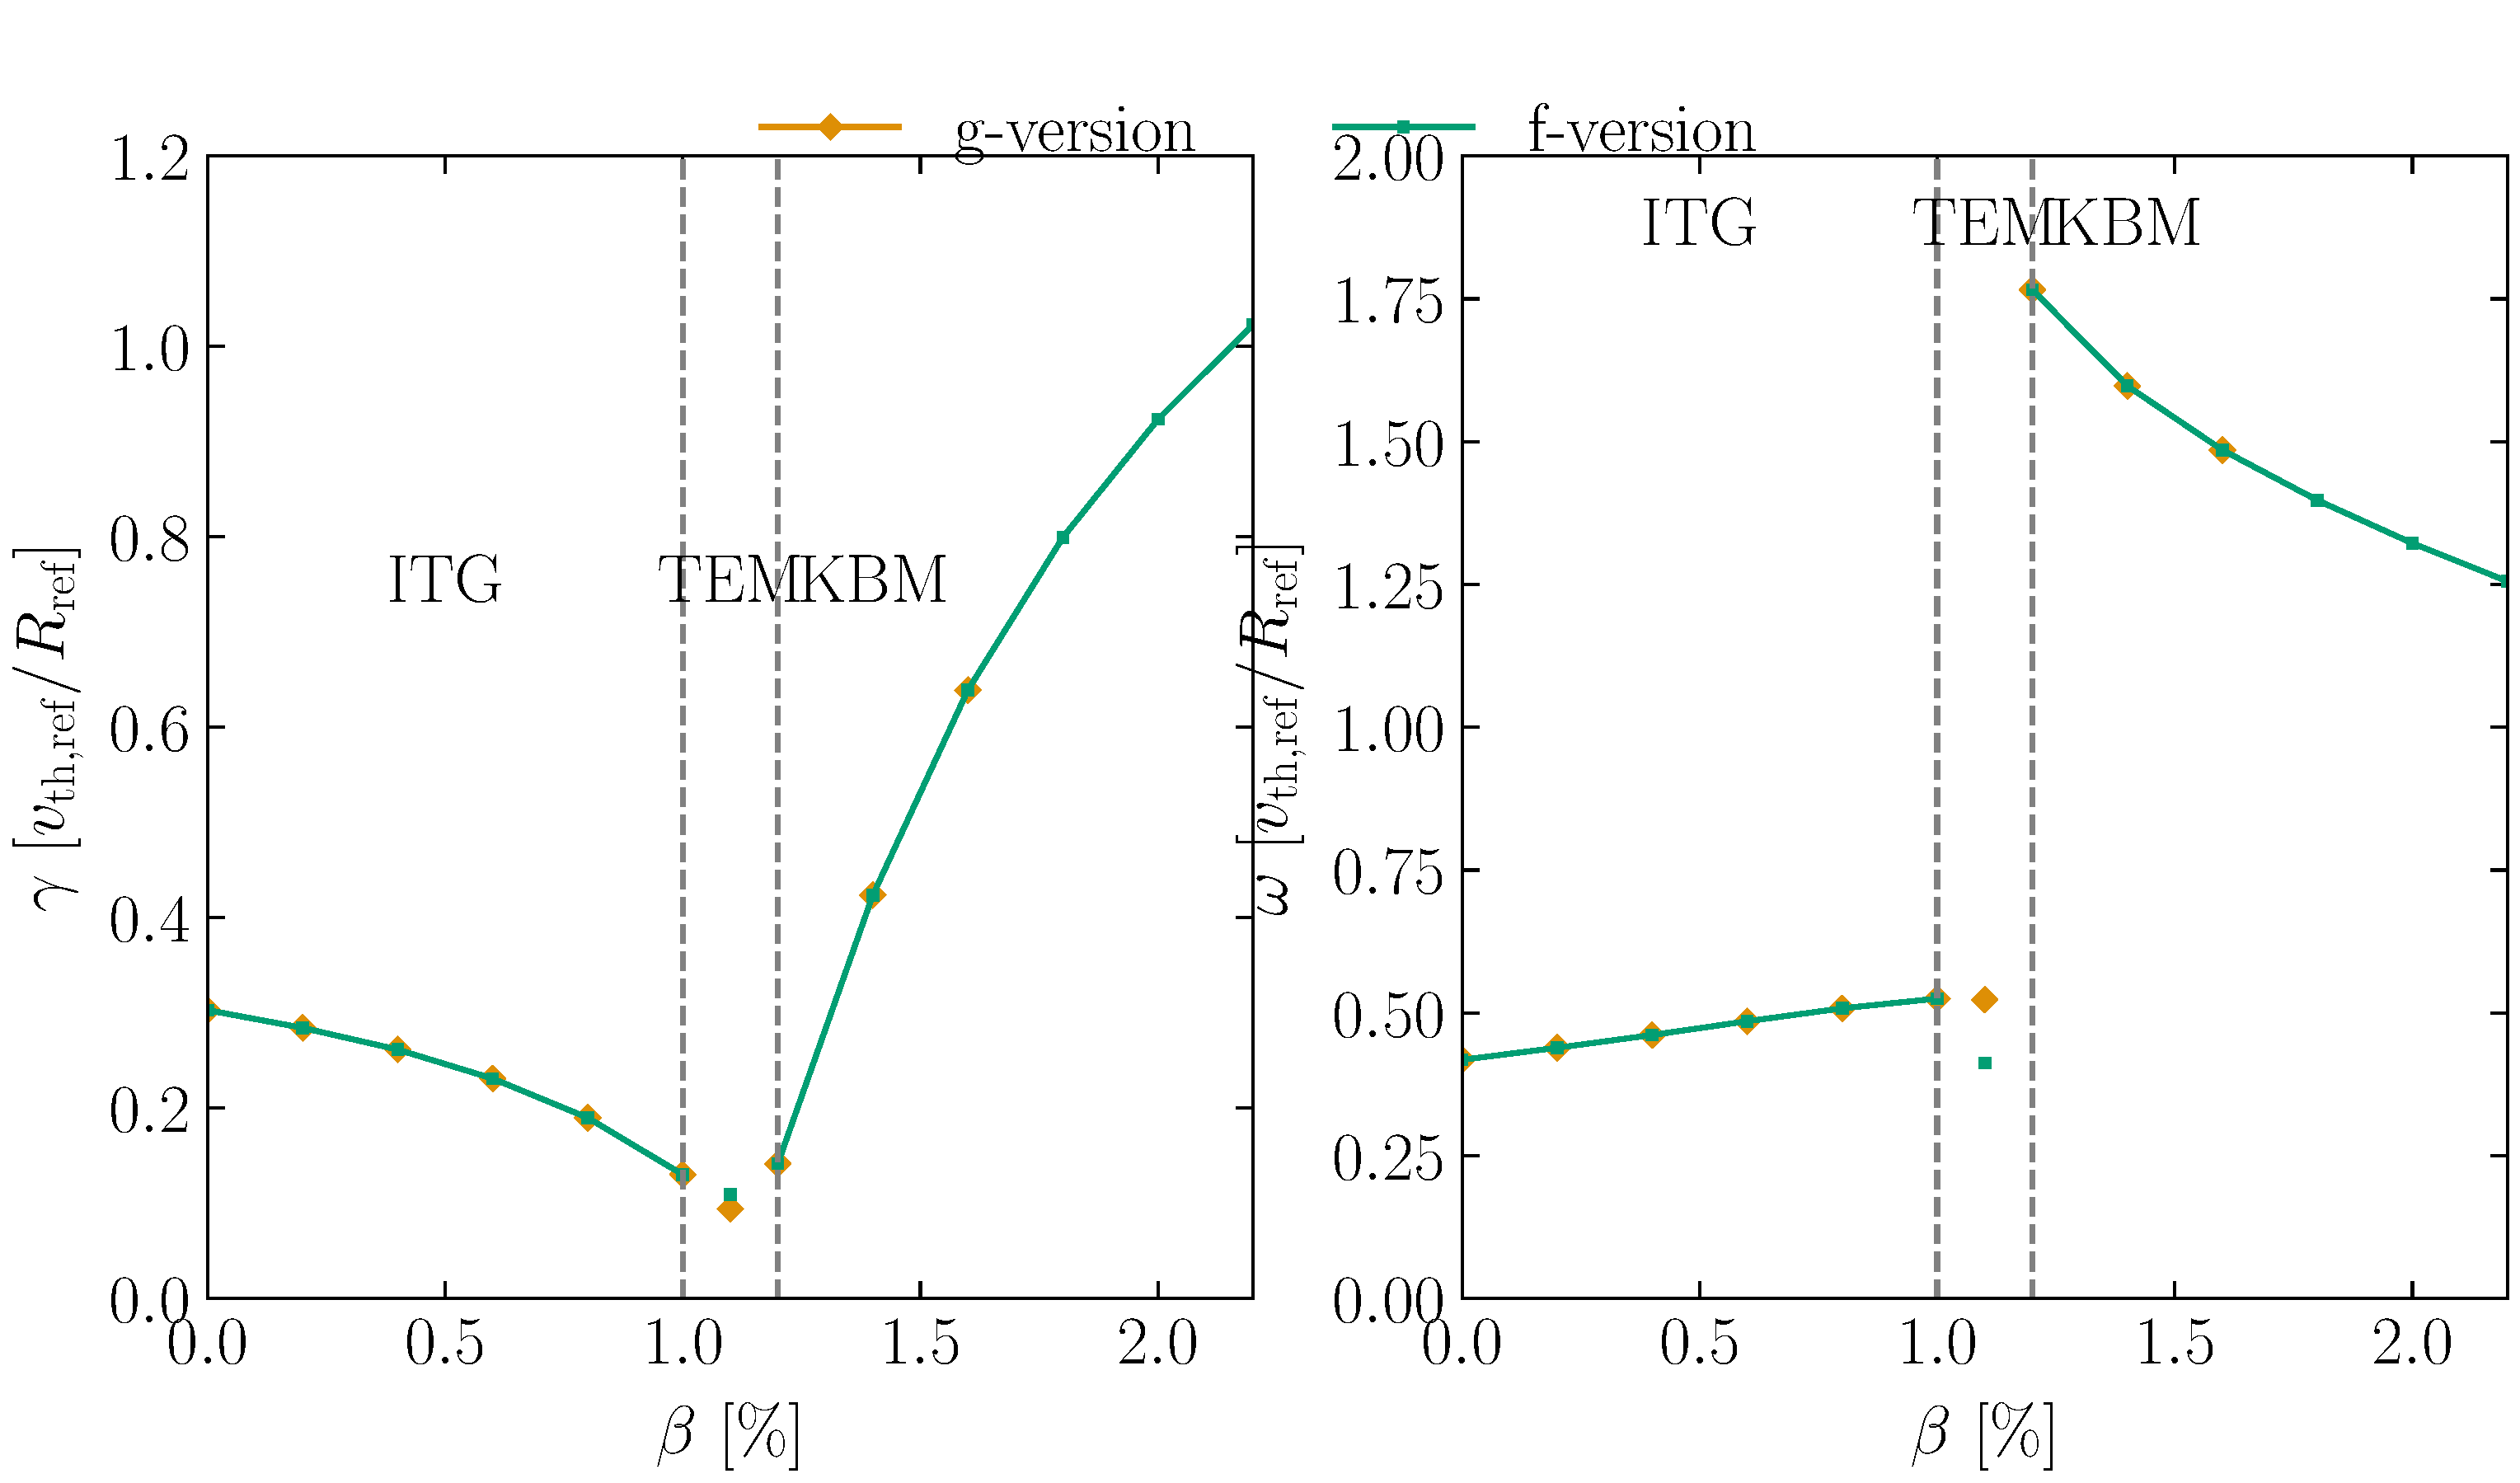
\includegraphics[height = 0.7\paperheight]{evaluation/benchmark/comparison/kthrho0.300_beta0.000-0.022_scan_comparison.pdf}\\ $10\,\%$ more runtime for the f-version}
		\only<4>{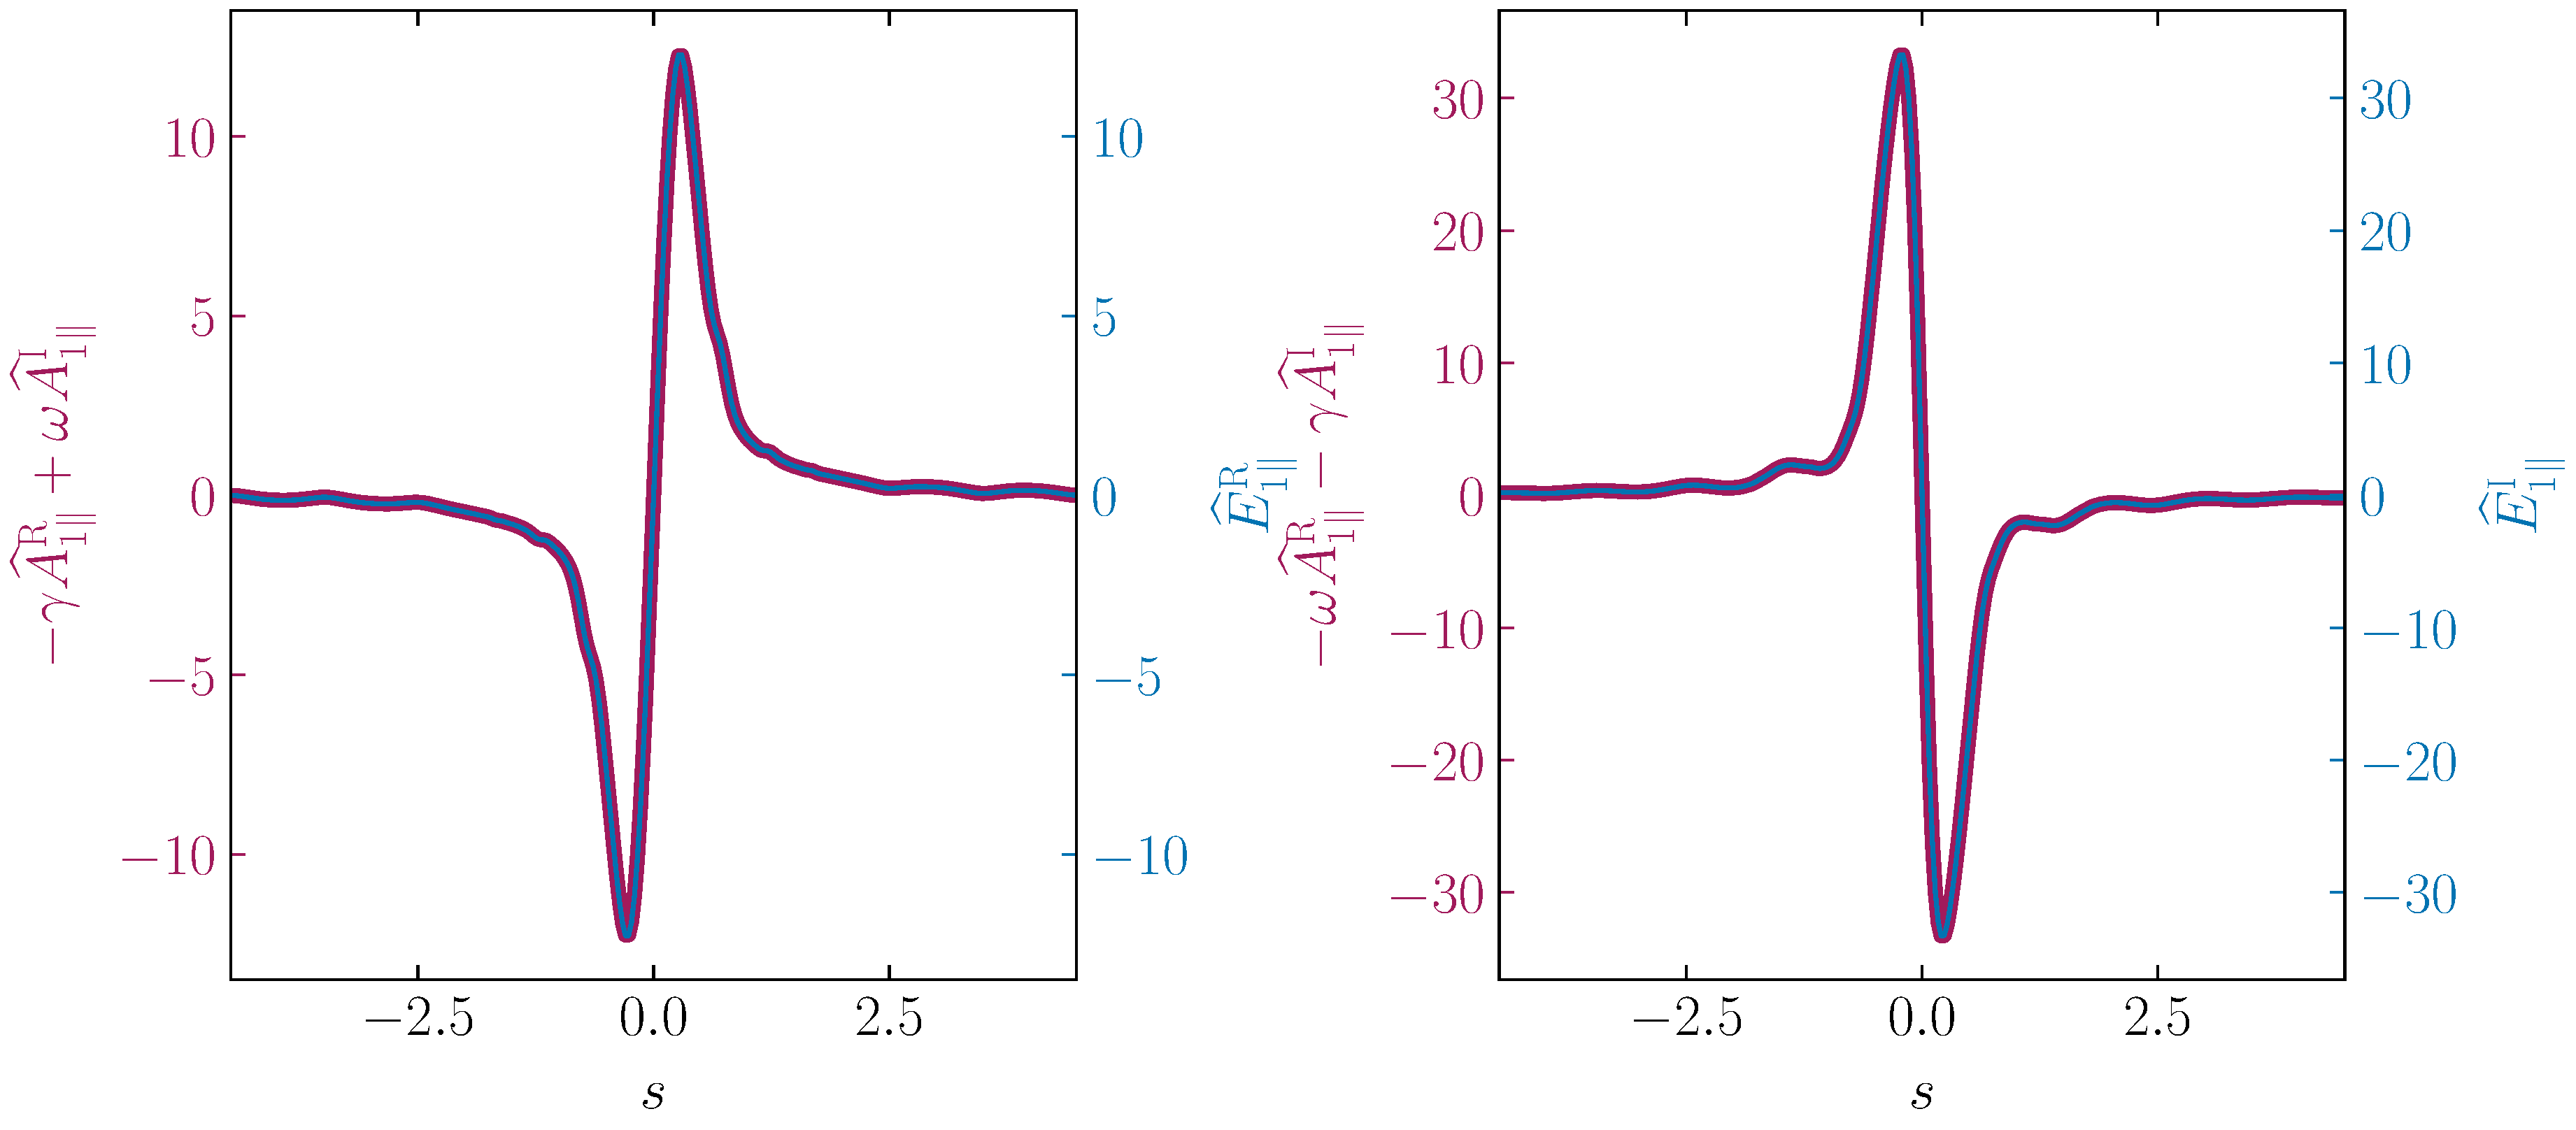
\includegraphics[width = 0.9\paperwidth]{evaluation/benchmark/f-version/fields/kthrho0.300_beta0.008_fields_f-version.pdf}\\ $\beta = 0.8\,\%$}
		\only<5>{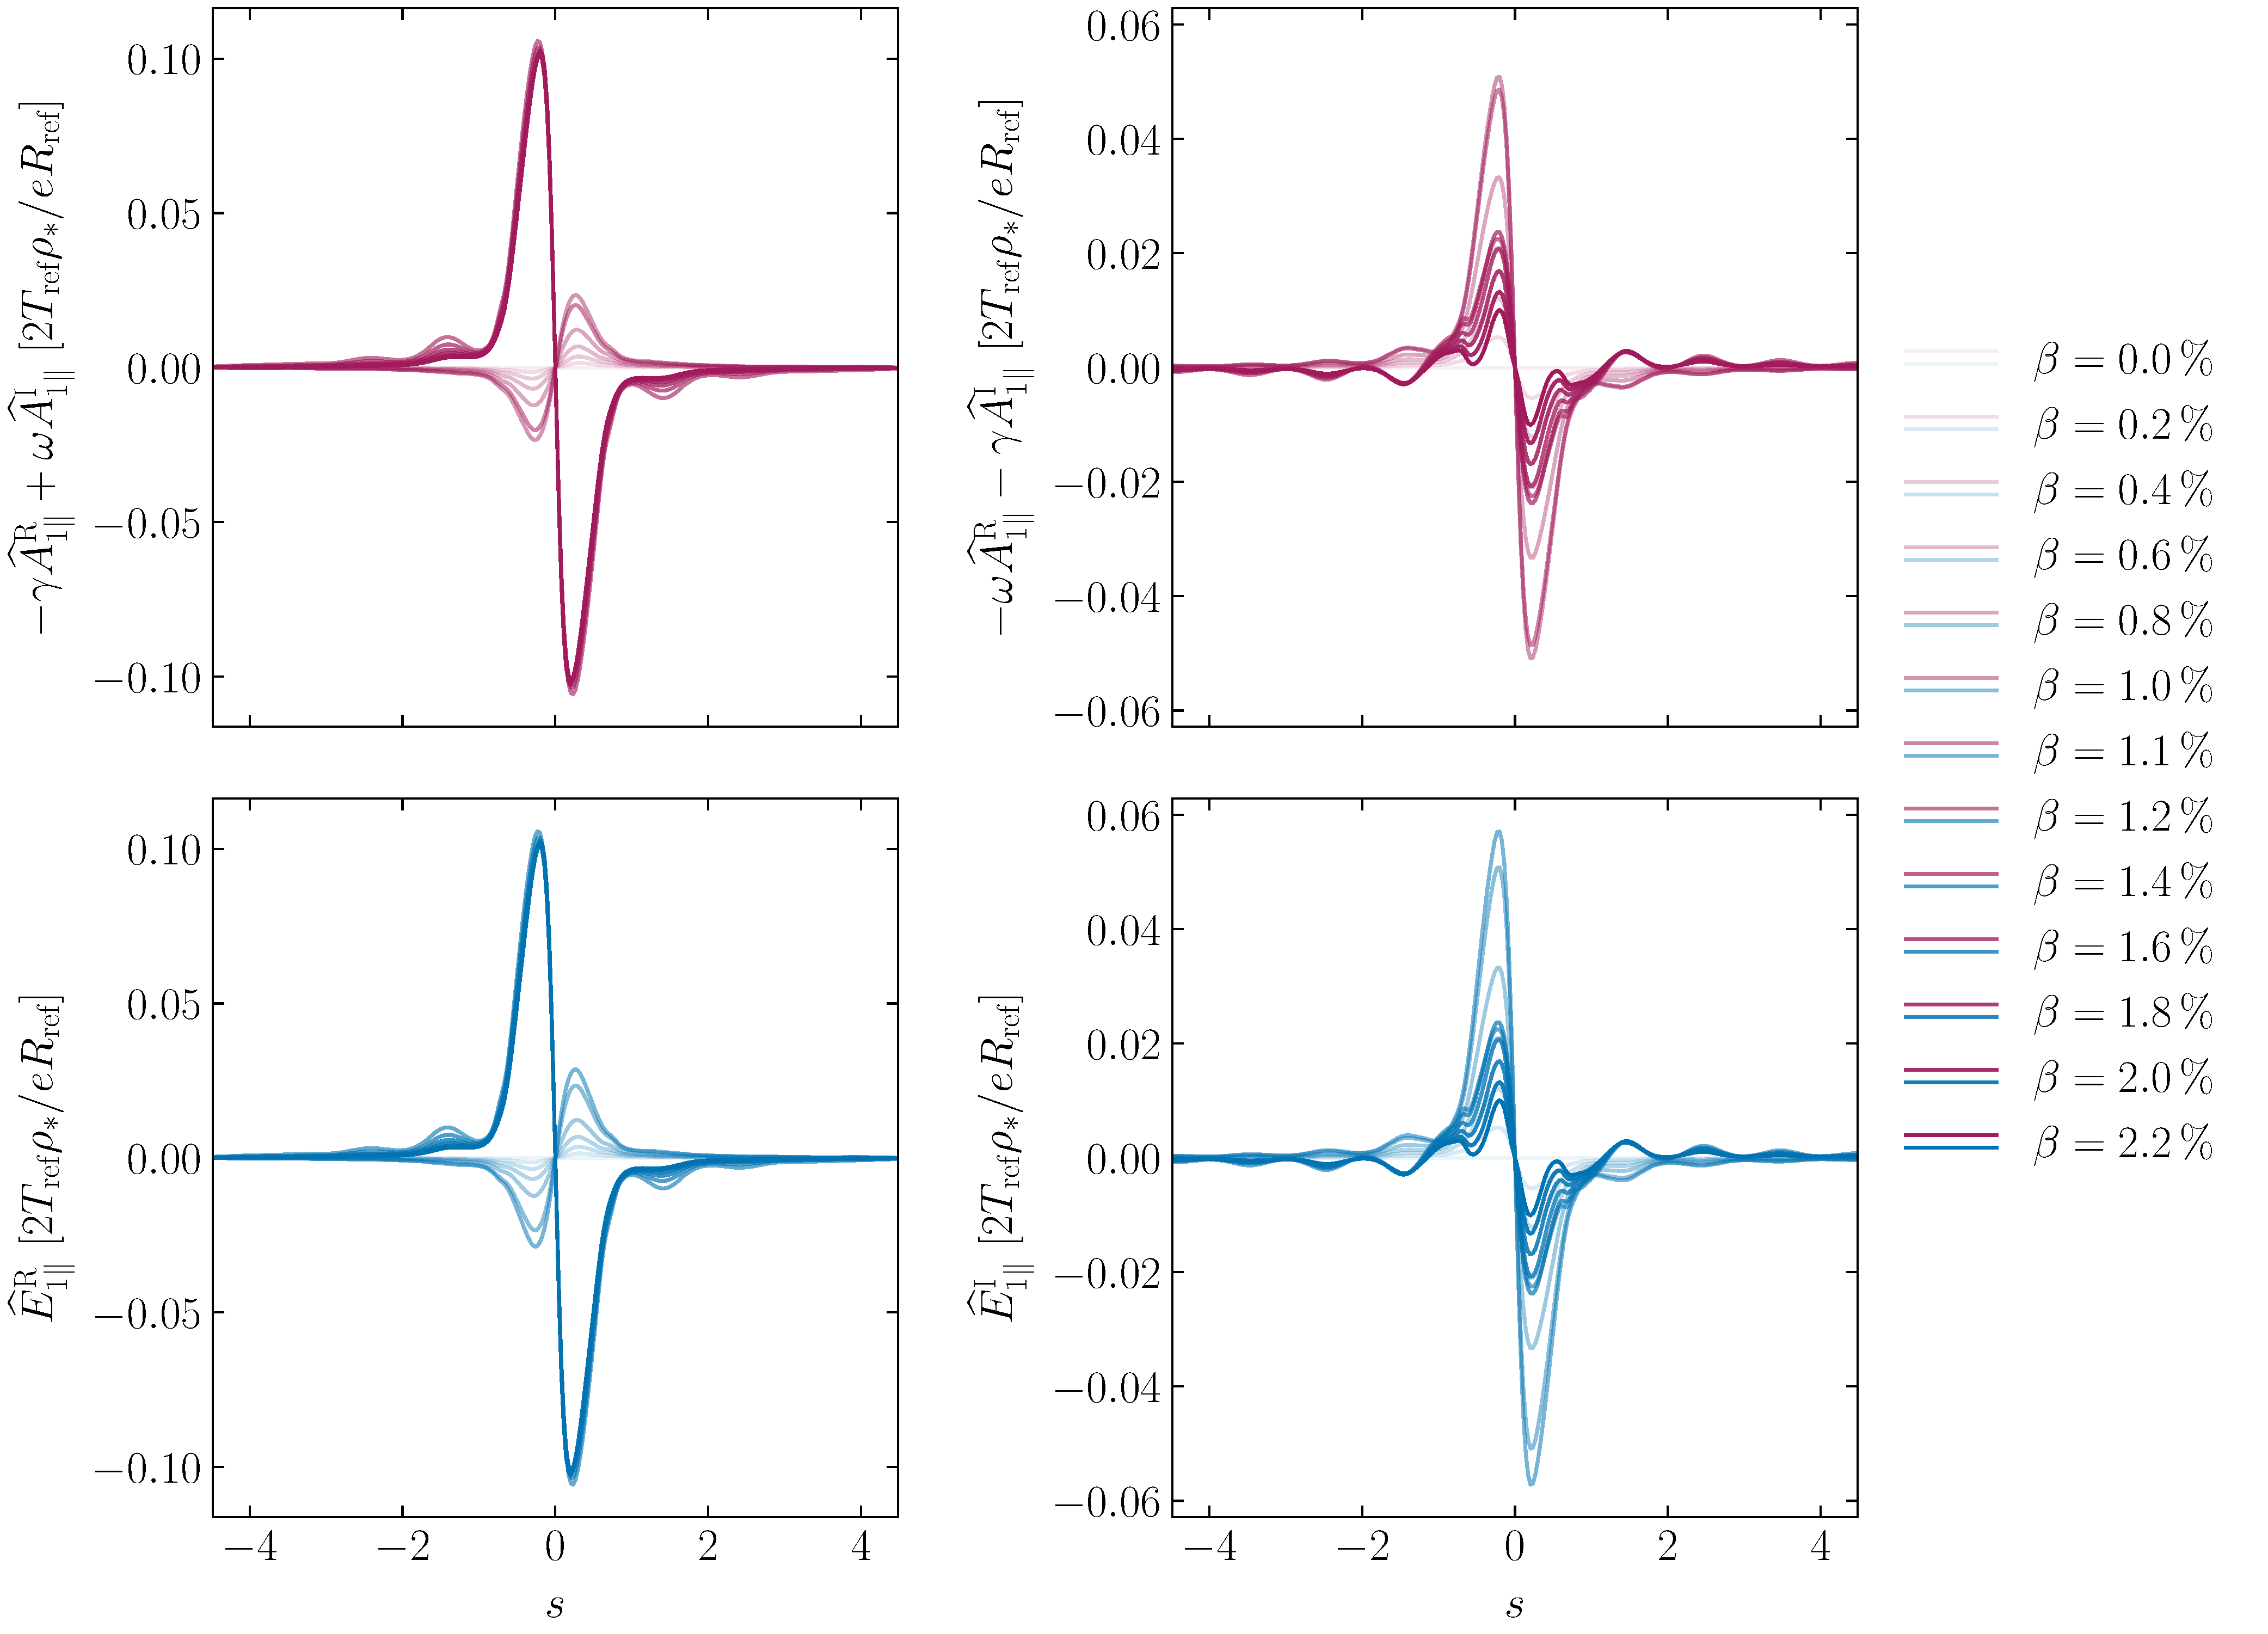
\includegraphics[height = 0.8\paperheight]{evaluation/benchmark/comparison/kthrho0.300_beta0.000-0.022_fields_f-version.pdf}}
	
	\end{frame}

	\begin{frame}
		\frametitle{Mitigation in local Simulations}
		
		\begin{center}
			\begin{itemize}
				\item <2-> Mitigation could only be tested in the local linear simulations \\ $\rightarrow$ Local nonlinear simulations not benchmarked yet
				\item <3-> CBC and AUG (ASDEX-Upgrade) test cases fails \\ for the same value of $\kperp$ in both versions
				\begin{align*}
					&\left(\kperpN^2 + \betaref \spec{\sum} \frac{\spec{Z^2}\specR{n}}{\specR{m}} \Gamma_0(\spec{b}) e^{-\specN{\cfen}/\specR{T}} \right) \FEparN = \\
					&- 2\pi\BN \betaref \spec{\sum} \spec{Z} \specR{n} \specthR{v} \ints \dvparN \dmuN ~ \vparN J_0(\kperp \spec{\rho}) \specN{\Frhs}
				\end{align*}
				\begin{align*}
					&\left(\kperpN^2 + \betaref \spec{\sum} \frac{\spec{Z^2}\specR{n}}{\specR{m}} \Gamma_0(\spec{b}) e^{-\specN{\cfen}/\specR{T}} \right) \FAparN = \\
					& 2\pi\BN \betaref \spec{\sum} \spec{Z} \specR{n} \specthR{v} \ints \dvparN \dmuN ~ \vparN J_0(\kperp \spec{\rho}) \specN{\widehat{g}}
				\end{align*}

			\end{itemize}
		\end{center}
	
	\end{frame}

	\section*{Conclusion}
	\begin{frame}
		\frametitle{Conclusion}
		
		\begin{center}
			\onslide<2->{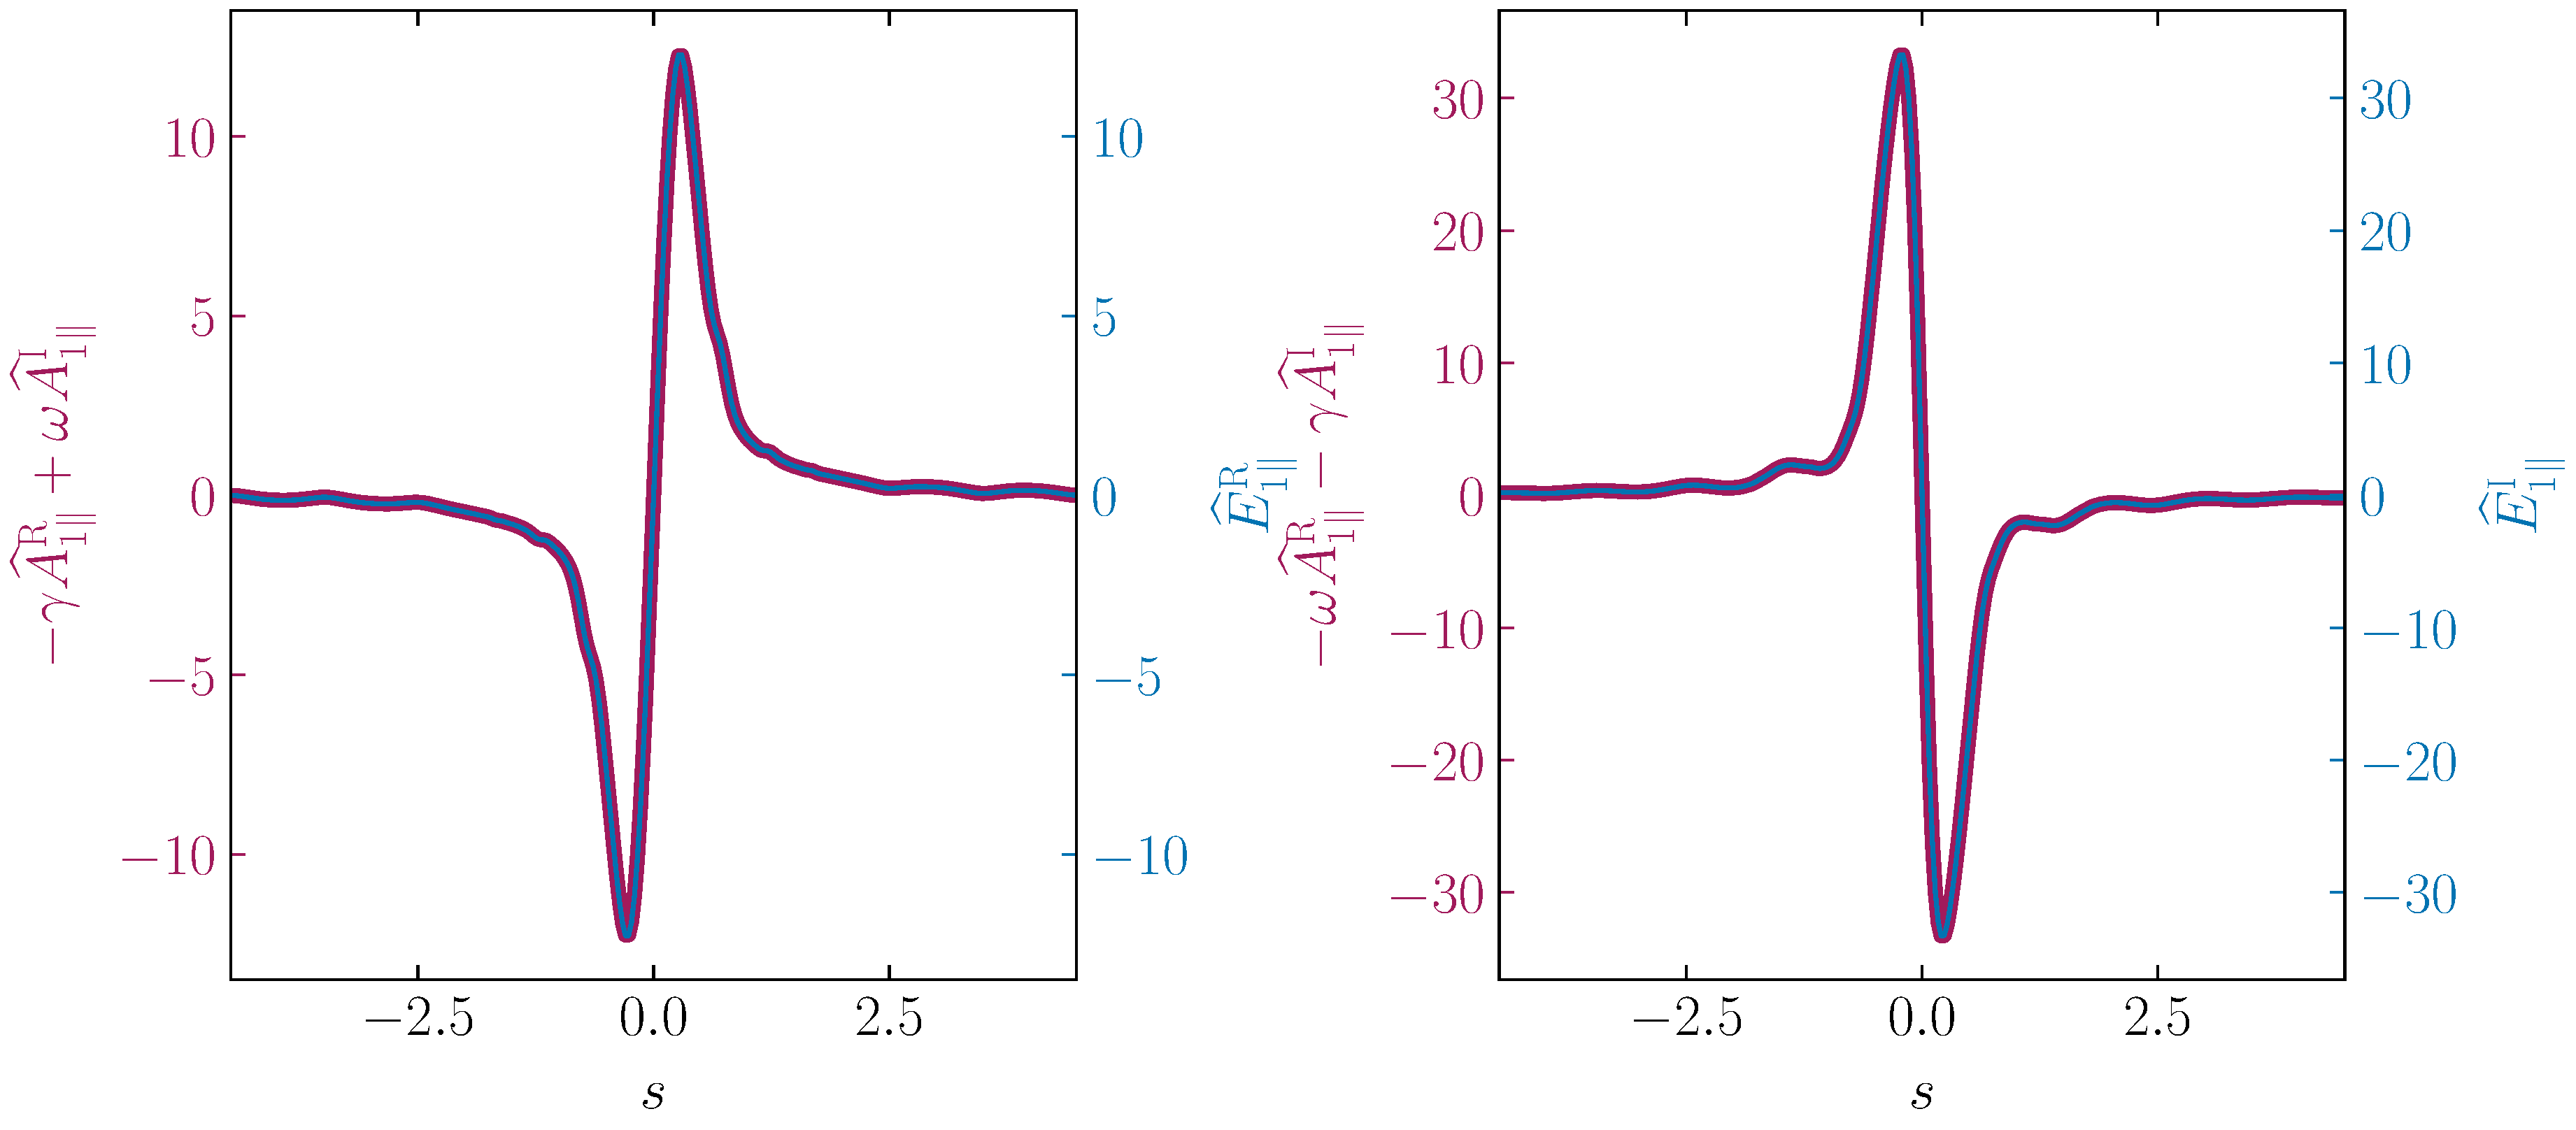
\includegraphics[width = 0.6\paperwidth]{evaluation/benchmark/f-version/fields/kthrho0.300_beta0.008_fields_f-version.pdf}}
			\begin{itemize}
				\item <2-> Local linear f-Version successfully implemented \\ $\rightarrow$ $10\,\%$ more runtime
				\item <3-> Nonlinear benchmark not completed yet
				\item <4-> Groundwork for global f-version of {\gkw} done
			\end{itemize}
		\end{center}
	
	\end{frame}

\end{document}